\section*{Runtime Analysis} % move the headers in a bit
\begin{itemize}
    % \item limit definitions \\
    % 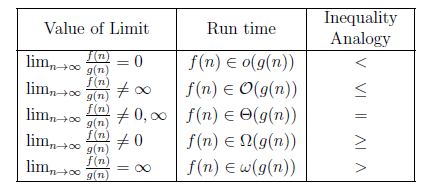
\includegraphics[scale = 1]{pictures/big o definition.png}
    \item big $O,~ \Omega,~ \Theta$ definition 
    \begin{align*}
        f &= O(g):~~\exists c, ~ \exists n_0~\text{ s.t }  n \geq n_0 \rightarrow f(n) \leq cg(n)\\
        f &= \Omega(g):~~ \exists c, ~\exists n_0 ~ \text{ s. t } n \geq n_0 \rightarrow f(n) \geq c g(n)\\
        &\rightarrow \text{ or } g \in O(f) \\
        f &= \Theta(g): ~~ f = O(g) \text{ and } f = \Omega(g)
    \end{align*}
    \item small $o, \omega$
    \begin{align*}
        f &= o(g): ~~ \forall c, ~ \exists n_0 ~ \text{ s.t } n \geq n_0 \rightarrow f(n) < c g(n) \\
        f &= \omega(g) ~~ \forall c, ~ \exists n_0 ~ \text{ s.t } n \geq n_0 \rightarrow f(n) > c g(n)
    \end{align*}
    \item small $o, \omega + \Theta$ limit definition
    \begin{align*}
        \lim_{n \rightarrow \infty} \frac{f(n)}{g(n)} = L~~
        \begin{cases}
            L = 0 \rightarrow f \in o(g) \\
            L = c \rightarrow f \in \Theta(g) \\
            L = \infty \rightarrow f \in w(g)
        \end{cases}
    \end{align*}
    \item big $O, \Omega$ limit definition
    \begin{align*}
        \lim_{n \rightarrow \infty} \frac{f(n)}{g(n)} = L ~~
        \begin{cases}
            L \neq \infty \rightarrow f \in O(g) \\
            L = \infty \rightarrow f \in \Omega(g)
        \end{cases}
    \end{align*}
    
    \item these are a list of common runtime (fastest $\rightarrow$ slowest in terms of runtime) 
    \end{itemize}
    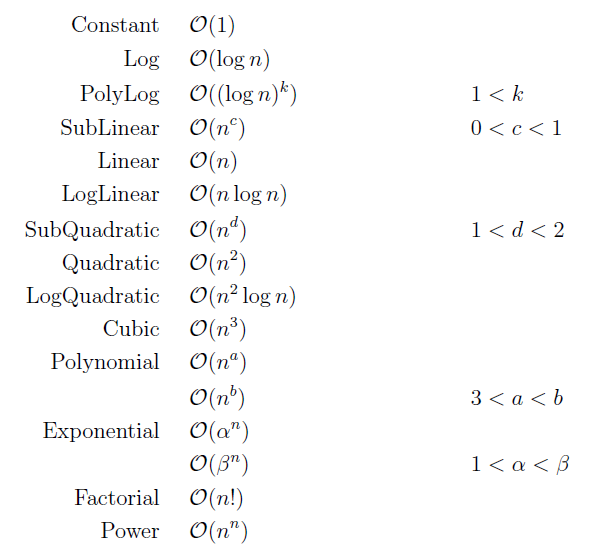
\includegraphics[scale = 0.7]{pictures/functions growth.png}
    \begin{itemize}
    \item important math/log rules
    \begin{align*}
        &c^{\log_c a} = a                   &&\log_a(x) > \log_b(x) \text{ if } a < b \\
        &\log_c (a \cdot b) = \log_c a + \log_c b           &&\log_c (b^k) = k \log_c b \\
        &\log_c (a / b) = \log_c a - \log_c b               &&\log_a b = {\log_c a}/{\log_c b}   \\
        % &&\log_c c = 1\\
        &C(n,r) = {n \choose r} = \frac{n!}{r!(n-r)!}              && P(n,r) = \frac{n!}{(n-r)!}
    \end{align*}
    % 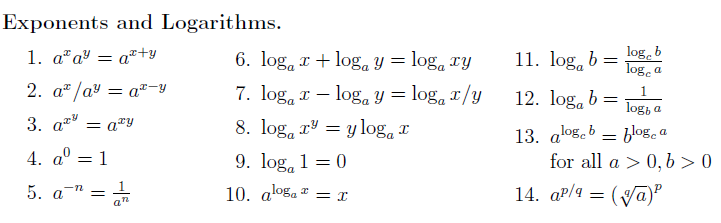
\includegraphics[scale = 0.7]{pictures/exponent and log.png}
    % \vfill\null 
    % \columnbreak 
    
\end{itemize}